\documentclass{article}
\usepackage[utf8]{inputenc}
\usepackage[greek,english]{babel}
\usepackage{alphabeta}
\usepackage{graphicx}
\usepackage{hyperref} 
\usepackage{listings}
\usepackage{subcaption}
\usepackage{mathtools}
\usepackage{amsmath}

\date{\vspace{-4ex}}
\title{Συστήματα Μικροϋπολογιστών}
\usepackage[svgnames]{xcolor} 
\newcommand*{\plogo}{\fbox{$\mathcal{PL}$}} 
\begin{document}

\begin{titlepage} % Suppresses displaying the page number on the title page and the subsequent page counts as page 1
	
	\raggedleft % Right align the title page
	
	\rule{1pt}{\textheight} % Vertical line
	\hspace{0.05\textwidth} % Whitespace between the vertical line and title page text
	\parbox[b]{0.75\textwidth}{ % Paragraph box for holding the title page text, adjust the width to move the title page left or right on the page
		
		{\Huge\bfseries Δίκτυα \\[0.5\baselineskip] Υπολογιστών ΙI}\\[2\baselineskip] % Title
		{\large\textit{ }}\\[4\baselineskip] % Subtitle or further description
		{\Large\textsc{Ιωάννης-Παναγιώτης \\Μπουντουρίδης}} %
	\\	\\{\large\textsc{ΑΕΜ: 8872}} % Author name, lower case for consistent small caps
		
		\vspace{0.5\textheight} % Whitespace between the title block and the publisher
		
		{\noindent \textit{report}}\\[\baselineskip] % Publisher and logo
	}

\end{titlepage}

\newpage


\section*{Πρωτόκολλο UDP }
Το πρωτόκολλο User Datagram Protocol (UDP) είναι ένα από τα βασικά πρωτόκολλα που χρησιμοποιούνται στο Διαδίκτυο. Μία εναλλακτική ονομασία του πρωτοκόλλου είναι Universal Datagram Protocol. Διάφορα προγράμματα χρησιμοποιούν το πρωτόκολλο UDP για την αποστολή σύντομων μηνυμάτων (γνωστών και ως datagrams) από τον έναν υπολογιστή στον άλλον μέσα σε ένα δίκτυο υπολογιστών.

Ένα από τα κύρια χαρακτηριστικά του UDP είναι ότι δεν εγγυάται αξιόπιστη επικοινωνία. Τα πακέτα UDP που αποστέλλονται από έναν υπολογιστή μπορεί να φτάσουν στον παραλήπτη με λάθος σειρά, διπλά ή να μην φτάσουν καθόλου εάν το δίκτυο έχει μεγάλο φόρτο. Χρησιμοποιείται όταν η "γρήγορη" παράδοση των πακέτων είναι πιο σημαντική από την "ακριβή" παράδοση, π.χ στη μετάδοση ομιλίας και βίντεο.. Αντιθέτως, το πρωτόκολλο TCP διαθέτει όλους τους απαραίτητους μηχανισμούς ελέγχου και επιβολής της αξιοπιστίας και συνεπώς μπορεί να εγγυηθεί την αξιόπιστη επικοινωνία μεταξύ των υπολογιστών. Η έλλειψη των μηχανισμών αυτών από το πρωτόκολλο UDP το καθιστά αρκετά πιο γρήγορο και αποτελεσματικό, τουλάχιστον για τις εφαρμογές εκείνες που δεν απαιτούν αξιόπιστη επικοινωνία.

Οι εφαρμογές audio και video streaming χρησιμοποιούν κατά κόρον πακέτα UDP. Για τις εφαρμογές αυτές είναι πολύ σημαντικό τα πακέτα να παραδοθούν στον παραλήπτη σε σύντομο χρονικό διάστημα ούτως ώστε να μην υπάρχει διακοπή στην ροή του ήχου ή της εικόνας. Κατά συνέπεια προτιμάται το πρωτόκολλο UDP διότι είναι αρκετά γρήγορο, παρόλο που υπάρχει η πιθανότητα μερικά πακέτα UDP να χαθούν. Στην περίπτωση που χαθεί κάποιο πακέτο, οι εφαρμογές αυτές διαθέτουν ειδικούς μηχανισμούς διόρθωσης και παρεμβολής ούτως ώστε ο τελικός χρήστης να μην παρατηρεί καμία αλλοίωση ή διακοπή στην ροή του ήχου και της εικόνας λόγω του χαμένου πακέτου. Σε αντίθεση με το πρωτόκολλο TCP, το UDP υποστηρίζει broadcasting, δηλαδή την αποστολή ενός πακέτου σε όλους τους υπολογιστές ενός δικτύου, και multicasting, δηλαδή την αποστολή ενός πακέτου σε κάποιους συγκεκριμένους υπολογιστές ενός δικτύου. Η τελευταία δυνατότητα χρησιμοποιείται πολύ συχνά στις εφαρμογές audio και video streaming ούτως ώστε μία ροή ήχου ή εικόνας να μεταδίδεται ταυτόχρονα σε πολλούς συνδρομητές.

Μερικές σημαντικές εφαρμογές που χρησιμοποιούν πακέτα UDP είναι οι εξής: Domain Name System (DNS), IPTV, Voice over IP (VoIP), Trivial File Transfer Protocol (TFTP) και τα παιχνίδια που παίζονται ζωντανά μέσω του Διαδικτύου. 
\section*{Δομή UDP πακέτου}
Η δομή ενός πακέτου UDP περιγράφεται αναλυτικά στο αντίστοιχο πρότυπο IETF RFC 768. Στην σουίτα πρωτοκόλλων του Διαδικτύου, το UDP βρίσκεται ανάμεσα στο επίπεδο δικτύου (network layer) και στο επίπεδο συνόδου (session layer) ή εφαρμογών (application layer).
Κάθε πακέτο UDP έχει μία κεφαλίδα (header) που αναφέρει τα χαρακτηριστικά του. Η κεφαλίδα περιλαμβάνει μονάχα 4 πεδία, τα οποία είναι πολύ λίγα εάν συγκριθούν με άλλα πρωτόκολλα, όπως το TCP. Δύο από τα τέσσερα πεδία είναι προαιρετικά (φαίνονται χρωματισμένα με ροζ). \clearpage
\begin{figure*}[h!]
 \begin{center}
  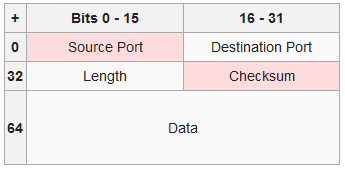
\includegraphics[width=50mm,scale=0.7]{pic1.png}
\end{center}
\end{figure*}
Ακολουθεί μία συνοπτική εξήγηση των πεδίων: \\
\textbf{Source port}
\par{Η πόρτα του αποστολέα από την οποία προήλθε το πακέτο. Εάν ο παραλήπτης επιθυμεί να στείλει κάποια απάντηση, θα πρέπει να την στείλει στην πόρτα αυτήν. Το συγκεκριμένο πεδίο δεν είναι υποχρεωτικό και στις περιπτώσεις που δεν χρησιμοποιείται θα πρέπει να έχει την τιμή μηδέν.}
\textbf{Destination port}
\par{Η πόρτα του παραλήπτη στην οποία θα πρέπει να παραδοθεί το πακέτο.} \\
\textbf{Length}
\par{Το πεδίο αυτό έχει μέγεθος 16-bit και περιλαμβάνει το μέγεθος του πακέτου σε bytes. Το μικρότερο δυνατό μέγεθος είναι 8 bytes, αφού η κεφαλίδα αυτή καθ' αυτή καταλαμβάνει τόσο χώρο. Θεωρητικά, το μέγεθος του UDP πακέτου δεν μπορεί να ξεπερνάει τα 65,527 bytes, αλλά πρακτικά το όριο μειώνεται στα 65,507 bytes λόγω διαφόρων περιορισμών που εισάγει το πρωτόκολλο IPv4 στο επίπεδο δικτύου.} \\
\textbf{Checksum} 
\par{    Ένα πεδίο 16-bit το οποίο χρησιμοποιείται για επαλήθευση της ορθότητας του πακέτου στο σύνολό του, δηλαδή τόσο της κεφαλίδας όσο και των δεδομένων. Στην συνέχεια το πακέτο UDP περνάει στο επίπεδο δικτύου, το οποίο αναλαμβάνει να το μεταδώσει στο δίκτυο υπολογιστών. Το επίπεδο αυτό τοποθετεί μία ακόμη κεφαλίδα στο πακέτο, η οποία διαφέρει ανάλογα με την έκδοση του πρωτοκόλλου που χρησιμοποιείται στο επίπεδο δικτύου (IPv4 ή IPv6). } \\
\textbf{Source Address, Destination Address }
\par{Οι διευθύνσεις IP του αποστολέα και του παραλήπτη αντίστοιχα.} \\
\textbf{Zeros} 
\par{Μία ακολουθία μηδενικών, η οποία δεν παίζει κανέναν ρόλο κατά την μετάδοση του πακέτου.} \\
\textbf{Protocol }
\par{Ένας χαρακτηριστικός αριθμός που αντιστοιχεί στο πρωτόκολλο που χρησιμοποιείται. Για το UDP η τιμή που παίρνει το πεδίο αυτό είναι 17.}\\
\textbf{Length} 
\par{    Το συνολικό μέγεθος του πακέτου. Στην συγκεκριμένη περίπτωση UDP length + IP Header length. Για IPv6, το πακέτο παίρνει την εξής μορφή:} \clearpage
\begin{figure*}[h!]
 \begin{center}
  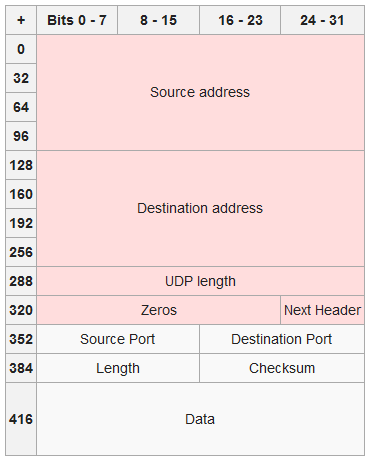
\includegraphics[width=50mm,scale=0.7]{pic2.png}
\end{center}
\end{figure*}
\textbf{Source Address, Destination Address }
\par{Οι διευθύνσεις IP του αποστολέα και του παραλήπτη αντίστοιχα, οι οποίες όμως στην περίπτωση αυτή είναι τύπου IPv6, δηλαδή πολύ μεγαλύτερες (IPv4 - 32bit, IPv6 - 128bit).
}\\
\textbf{UDP Length }
\par{Το συνολικό μέγεθος του πακέτου UDP, όπως και προηγουμένως.}\\
\textbf{Zeros }
\par{Μία ακολουθία μηδενικών, η οποία δεν παίζει κανέναν ρόλο κατά την μετάδοση του πακέτου.}\\
\textbf{Next Header }
\par{Το πεδίο αυτό παίρνει μία τιμή που είναι χαρακτηριστική για το πρωτόκολλο που χρησιμοποιείται. Στην περίπτωση του UDP, η τιμή αυτή είναι 17. Στην περίπτωση IPv6 το πεδίο checksum του UDP πακέτου δεν είναι πλέον προαιρετικό, αλλά θα πρέπει υποχρεωτικά να συμπληρωθεί.}
\clearpage
\section*{Audio streaming Protocols}
Οι audio streaming εφαρμογές, που ανήκουν στην κατηγορία των streaming media, είναι ένα είδος εφαρμογών που χαρακτηρίζονται από τη συνεχή ροή δεδομένων, καθώς και τη συνεχή αναπαραγωγή τους στον τελικό χρήστη με τη μορφή ήχου, σχεδόν αμέσως κατά την άφιξή τους στον τελικό προορισμό τους.

Αυτή είναι και η κυριότερη διαφορά των streaming media σε σχέση με πιο “παραδοσιακά” μέσα μετάδοσης πληροφοριών, όπως τα CDs και οι κασέτες.
Επίσης, ο όρος αποδίδεται κυρίως στη μεταφορά πληροφοριών μέσω τηλεπικοινωνιακών δικτύων, διαχωρίζοντας έτσι αυτήν την κατηγορία από την παραδοσιακή τηλεόραση και το ραδιόφωνο.

Προκειμένου να γίνει εφικτή η υλοποίηση των streaming media και ειδικότερα των audio streaming εφαρμογών, σχεδιάστηκαν αρκετά πρωτόκολλα που τυποποιούν όλες τις απαραίτητες διαδικασίες.

Τα βασικότερα ίσως πρωτόκολλα είναι ίσως τα datagram πρωτόκολλα, όπως το UDP (User Datagram Protocol), σύμφωνα με το οποίο η αποστολή των δεδομένων υλοποιείται με μία ροή μικρών πακέτων δεδομένων.
Παρόλο που αυτή η ιδέα είναι απλή και αποτελεσματική, πρέπει να λαμβάνεται υπόψη το γεγονός ότι τα πακέτα μπορούν εν δυνάμει να χαθούν ή να αλλοιωθούν κατά τη μεταφορά τους κατά μήκος του δικτύου.
Ανάλογα με το χρησιμοποιούμενο πρωτόκολλο και την τάξη των απωλειών των πακέτων, τα δεδομένων στην πλευρά του τελικού χρήστη μπορούν να ανακτηθούν με ανάπτυξη, σε επίπεδο εφαρμογής, ειδικών τεχνικών διόρθωσης σφαλμάτων για αλλοιωμένα πακέτα, τεχνικών παρεμβολής ώστε να μη γίνεται αισθητή η ολοκληρωτική καταστροφή πακέτων, ειδάλλως ο τελικός χρήστης αναγκάζεται να υποστεί μέχρι και στιγμιαία διακοπή της αναπαραγωγής του ήχου στις audio streaming εφαρμογές, ακριβώς επειδή διακόπτεται και η ροή δεδομένων προς αυτών με την απώλεια κάποιων πακέτων.
Το RTSP είναι ένα πρωτόκολλο που επιτρέπει έναν client να χειρίζεται από απόσταση έναν streaming media server, με τη χρήση εντολών σαν αυτές που συναντώνται στις οικιακές συσκευές ψυχαγωγίας, όπως “play” ή “pause”, και κάνει εφικτή την time-based πρόσβαση σε αρχεία σε έναν server.
Το RTP καθορίζει ένα συγκεκριμένο format πακέτων για τη μετάδοση ήχου και video στο internet.

Δεν λειτουργεί σε μία συγκεκριμένη TCP ή UDP πόρτα, αλλά ο μόνος περιορισμός που υπάρχει είναι ότι η UDP επικοινωνία λαμβάνει χώρα διαμέσου μίας άρτιας πόρτας, ενώ η αμέσως επόμενη περιττή πόρτα δεσμεύεται σύμφωνα με το RTCP.
Συμπεραίνουμε λοιπόν, ότι το RTP συναντάται σε συνδυασμό με το RTCP, και “λειτουργούν” πάνω στο UDP.
Συνήθως το RTP χειρίζεται real-time δεδομένα, όπως interactive ήχος και video.
Έτσι, συναντάται συχνά σε εφαρμογές videoconferencing ή Voice over IP.
Οι εφαρμογές που βασίζονται στο RTP είναι γενικά λιγότερο ευαίσθητες στην απώλεια πακέτων, αλλά σχετικά ευαίσθητες στην καθυστέρηση άφιξης των πακέτων, έτσι το UDP είναι πολύ καλύτερη επιλογή από το TCP για τέτοιου είδους εφαρμογές.
Το πρωτόκολλο δεν παρέχει μηχανισμούς εξασφάλισης της επιτυχούς παράδοσης των πακέτων, ενώ και η παράδοσή τους σε λανθασμένη σειρά είναι πιθανή.
Επίσης δεν παρέχονται εγγυήσεις Quality of service, αν και όλα αυτά μπορούν να εξασφαλιστούν με κάποιον άλλον τρόπο (πχ το πρωτόκολλο δίνει όλα τα εφόδια ώστε να αναπτυχθεί σε επίπεδο εφαρμογής μηχανισμός που να αναδιατάσσει σε σωστή σειρά τα αφιχθέντα πακέτα).

Το RTCP είναι το “αδελφό” πρωτόκολλο του RTP, καθώς όπως προαναφέρθηκε συναντώνται πάντα σε συνδυασμό, και παρέχει διάφορες πληροφορίες που κάνουν δυνατό τον έλεγχο της ροής δεδομένων που βασίζεται στο RTP.
Δηλαδή, παρόλο που “συμπληρώνει” το RTP κατά την κατάτμηση σε πακέτα και τη μεταφορά των multimedia δεδομένων, δε μεταφέρει το ίδιο δεδομένα.
Χρησιμοποιείται ώστε να μεταδοθούν περιοδικά πακέτα ελέγχου στους συμμετέχοντες σε μία streaming media σύνοδο.
Κύρια λειτουργία του είναι να παρέχει ένα είδος feedback σχετικά με το quality of service που παρέχεται από το RTP.
Έτσι, συλλέγει στατιστικά δεδομένα μίας media σύνδεσης, και πληροφορίες όπως τα απεσταλμένα bytes, τα απεσταλμένα πακέτα, τα χαμένα – κατεστραμμένα πακέτα, το jitter, ο χρόνος απόκρισης, κ.ά.
Μια εφαρμογή μπορεί να χρησιμοποιήσει αυτές τις πληροφορίες ώστε να βελτιώσει το quality of service που παρέχεται, με τον πιθανό περιορισμό της ροής δεδομένων, ή της χρήσης ενός codec χαμηλής αντί υψηλής συμπίεσης.

Σε αντίθεση με το UDP, υπάρχουν πιο αξιόπιστα πρωτόκολλα, όπως το TCP, το οποίο μπορεί να εγγυηθεί την επιτυχή μετάδοση και παράδοση κάθε bit της ροής των media δεδομένων.
Παρόλα αυτά, αυτό επιτυγχάνεται μέσω ενός συστήματος με timeouts και επανεκπομπές πακέτων, που το κάνει ιδιαίτερο πολύπλοκο στην υλοποίηση.
Επίσης, όταν έχουμε καταστροφή και απώλεια ενός πακέτου κατά τη διαδρομή του στο διαδίκτυο, οι μηχανισμοί αυτοί συνεπάγονται τη διακοπή της ροής των δεδομένων έτσι ώστε να γίνει αντιμετώπιση αυτής της απώλειας με επανεκπομπή του χαμένου πακέτου.
Η εφαρμογή του τελικού χρήστη μπορεί να καταπολεμήσει το ενδεχόμενο της διακοπτόμενης ροής δεδομένων με τη χρήση μνήμης buffer, ώστε να μη διακόπτεται η αναπαραγωγή του ήχου προς το χρήστη.

Παρατηρούνται επίσης οι εξής κατηγορίες πρωτοκόλλων

Σύμφωνα με τα unicast πρωτόκολλα ο server αποστέλλει προς τον κάθε client ένα ξεχωριστό αντίγραφο του media stream.
Σαν ιδέα μπορεί να είναι απλό, αλλά στην πράξη μπορεί να οδηγήσει στην μαζική κυκλοφορία αυτών των δεδομένων στο δίκτυο.

Αντίθετα, τα multicast πρωτόκολλα στέλνουν μόνο ένα αντίτυπο της media ροής μέσω μίας οποιασδήποτε σύνδεσης, για παράδειγμα στη διαδρομή άμεσα σε δύο routers του δικτύου.
Αυτός είναι ένας πιο αποτελεσματικός τρόπος εκμετάλλευσης της χωρητικότητας του δικτύου, αλλά πολύ πιο πολύπλοκος στην υλοποίηση.

Ένα από τα πιο σημαντικά multicast πρωτόκολλα, το IP πρωτόκολλο, πρέπει να υλοποιηθεί σε όλους τους κόμβους που μεσολαβούν ανάμεσα στο server και στον client, συμπεριλαμβανομένων και των router του δικτύου.
Σύμφωνα με αυτό, αναπτύχθηκε μία μέθοδος προώθησης IP datagrams σε ένα γκρουπ ενδιαφερομένων παραληπτών – clients.
Από το 2005 όμως, οι περισσότεροι routers στο internet δεν υποστηρίζουν το IP multicast, και πολλά firewalls το μπλοκάρουν.
Το IP multicast είναι πιο πρακτικό για οργανισμούς που αναπτύσσουν τα δικά τους δίκτυα, όπως πανεπιστήμια και εταιρίες, καθώς, απ’ τη στιγμή που στήνουν ιδιόκτητα routers και συνδέσμους δικτύου, μπορούν να αποφασίσουν κατά πόσο το οικονομικό κόστος και η όλη προσπάθεια της υποστήριξης του IP multicast αξίζει σε σχέση με την τελική οικονομία στο bandwidth.

Τα P2P (Peer-to-peer) πρωτόκολλα ορίζουν ένα νέο τρόπο μετάδοσης των δεδομένων, σύμφωνα με τον οποίο αυτά μεταδίδονται από clients που τα έχουν ήδη, προς clients που δεν τα έχουν και τα επιθυμούν.
Αυτό αποτρέπει το server και τις δικτυακές του συνδέσεις από το φαινόμενο bottleneck.
Παρόλα αυτά, ανακύπτουν τεχνικά θέματα, θέματα απόδοσης, ποιότητας, ενώ πολύ σοβαρά είναι επίσης και τα νομικά θέματα, όπως έχει διαφανεί τα τελευταία χρόνια.

Παρακάτω έχουμε μία εισαγωγική αναφορά στον εξοπλισμό που χρησιμοποιήθηκε στην εργασία, που μπορεί να επηρεάζει τις μετρήσεις που διεξάγονται (px bandwidth σύνδεσης), ενώ έπειτα ακολουθεί το κύριο μέρος της εργασίας.
\end{document}